\documentclass{article}
\usepackage{gvv-book}
\usepackage{gvv}
\usepackage{amsmath}
\usepackage{amsfonts}
\usepackage{tikz}
\usepackage{setspace}
\usepackage{gensymb}
\usepackage[cmex10]{amsmath}
\usepackage{amsthm}
\usepackage{mathrsfs}
\usepackage{txfonts}
\usepackage{stfloats}
\usepackage{bm}
\usepackage{cite}
\usepackage{cases}
\usepackage{subfig}
\usepackage{longtable}
\usepackage{multirow}
\usepackage{enumitem}
\usepackage{mathtools}
\usepackage{tikz}
\usepackage{circuitikz}
\usepackage{verbatim}
\usepackage[breaklinks=true]{hyperref}
\usepackage{tkz-euclide}
\usepackage{listings}
\usepackage{color}    
\usepackage{array}    
\usepackage{longtable}
\usepackage{calc}     
\usepackage{multirow} 
\usepackage{hhline}   
\usepackage{ifthen}   
\usepackage{lscape}     
\usepackage{chngcntr}
\usepackage{graphicx}
\usepackage{float}
\usepackage{multicol}
\usepackage[a4paper, left = 1.5cm, right = 1.5cm]{geometry}



\begin{document}

\begin{center}
\large
    \textbf{Samyak Gondane-AI25BTECH11029}
\end{center}
\date{}

\section*{Question}
Find the angle between two vectors $\vec{a}$ and $\vec{b}$ with magnitudes 1 and 2 respectively and when $\vec{a}\cdot\vec{b} = 1$.

\section*{Solution}
Given two vectors $\vec{a}$ and $\vec{b}$ with magnitudes:


\begin{align}
\|\vec{a}\| = 1, \quad \|\vec{b}\| = 2
\end{align}


and dot product:


\begin{align}
\vec{a} \cdot \vec{b} = 1
\end{align}



We use the matrix formulation of the dot product:


\begin{align}
\vec{a} \cdot \vec{b} = \vec{a}^T \vec{b} = \|\vec{a}\| \|\vec{b}\| \cos\theta
\end{align}



Substituting the known values:


\begin{align}
1 = (1)(2)\cos\theta \Rightarrow \cos\theta = \frac{1}{2}
\Rightarrow \theta = \cos^{-1}\left(\frac{1}{2}\right)
\Rightarrow \theta = 60^\circ
\end{align}



\section*{Matrix Representation}

Let:


\begin{align}
\vec{a} = \myvec{1 \\ 0}, \quad
\vec{b} = \myvec{1 \\ \sqrt{3}}
\end{align}



Then:


\begin{align}
\vec{a}^T \vec{b} = 1
\end{align}




\begin{align}
\|\vec{a}\| = \sqrt{1^2 + 0^2} = 1, \quad
\|\vec{b}\| = \sqrt{1^2 + {\sqrt{3}}^2} = 2
\end{align}



So the angle is:


\begin{align}
\theta = \cos^{-1}\left(\frac{\vec{a}^T \vec{b}}{\|\vec{a}\| \|\vec{b}\|}\right)
= \cos^{-1}\left(\frac{1}{2}\right) = 60^\circ
\end{align}

\begin{figure}[H]
    \centering
    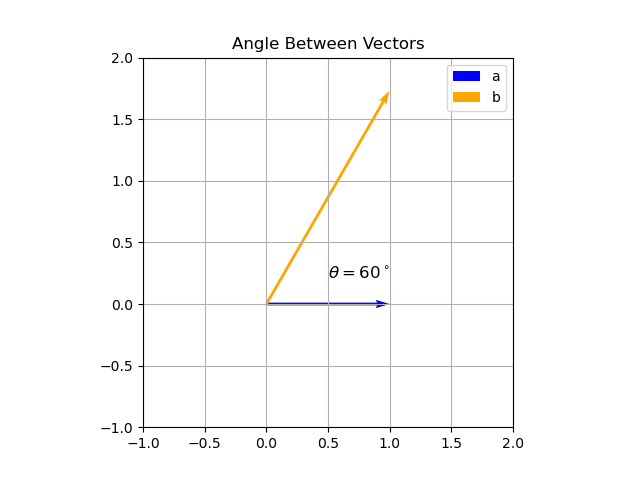
\includegraphics[width=0.7\linewidth]{figs/Figure_1.png}
    \caption{}
    \label{fig:fig1}
\end{figure}


\end{document}
